\documentclass[11pt,letterpaper]{article}

\usepackage[letterpaper,margin=0.8in,nohead]{geometry}

\usepackage[colorlinks]{hyperref}
\usepackage{url}
\usepackage{breakurl}

\hypersetup{
	colorlinks,
	linkcolor={red},
	citecolor={red},
	urlcolor={blue}
}

\usepackage{verbatim}
\usepackage{fancyvrb}
\usepackage{scrextend}
\usepackage{enumitem}
\usepackage{url}
\usepackage{tabularx}
\usepackage{float}

\usepackage{caption}
\usepackage{graphicx}
\usepackage{subcaption}

\usepackage{changepage}   % for the adjustwidth environment

\newenvironment{answer}{\em \color{blue} \begin{adjustwidth}{1cm}{1cm}}{\end{adjustwidth}}

% math
\usepackage{amsthm,amsmath}
\usepackage{amsfonts}

\newcommand{\mc}[1]{\mathcal{#1}}	% Mechanisms / Algorithms
\newcommand{\rv}[1]{\mathbf{#1}}    % Random variable

\newcommand{\pr}[1]{\mathrm{Pr}\{#1\}} % Probability

\newtheorem{corollary}{\bf Corollary}%[theorem]
\newtheorem{lemma}{\bf Lemma}%[theorem]
\newtheorem{definition}{\bf Definition}%[section]

\newtheorem{observation}{\bf Observation}%[theorem]

% load cleveref last!
\usepackage[capitalise]{cleveref}


\begin{document}
	
	\title{EN4720: Security in Cyber-Physical Systems \\ Exercise --- Infrastructure Security}
	
	%% This is an individual assignment!!
	%% TODO: put your name and index number here here!
	\author{ \textcolor{blue}{Name: Thalagala B. P.} \\ \textcolor{blue}{Index No: 180631J}}
	
	\maketitle
	
	\begin{center}
		\color{red}\bf This is an individual exercise! \\ Due Date: 20 June 2023 by 11.59 PM
	\end{center}
	
	% \begin{center}
		%     \small Content adopted from the Udacity Security Engineer Nano-Degree
		% \end{center}
	
	\vspace{1in}
	
	This exercise has to be carried out using a Linux-based PC/virtual machine. Read all the instructions and questions before attempting the exercise. Add answers under each question and submit the resulting PDF.
	
	
	\newpage
	\section*{Section 1}
	
	In this section, you will implement Firewall rules using \textbf{iptables} and \textbf{ufw} Linux commands. Moreover, you will scan network ports of a remote device using \textbf{nmap} Linux command.  
	
	For all the questions in this section, add a screenshot of the terminal (including all the commands you ran to perform the task) unless specified otherwise. The evaluator should be able to see each step that you followed to perform each task. In all screenshots, the areas marked (which are unique to your terminal display) in Figure 1 (the sample answer to Question 1) must be visible.
	
	\begin{enumerate}
		
		\item View the currently logged in user.
		
		\begin{figure}[H]
			\centering
			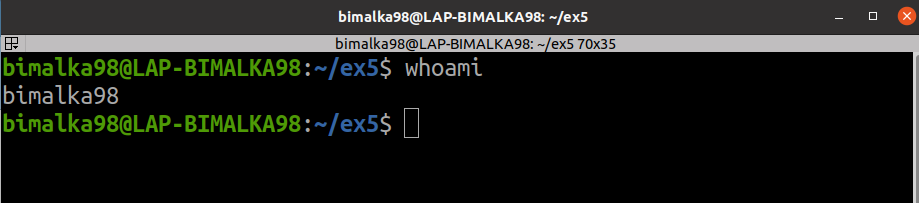
\includegraphics[width=0.65\columnwidth]{images/part1/1.png}
			\caption{Currently logged-in user} \label{fig:1}
		\end{figure}
		
		\subsubsection*{Creating Firewall Rules with iptables}
		
		\item Use \texttt{dpkg -l \textbar \ grep iptables} command to check whether iptables is installed on your system. If it does not existing in your system, install it by running \texttt{sudo apt-get install iptables}.
		
		\begin{answer}
			\begin{figure}[H]
				\centering
				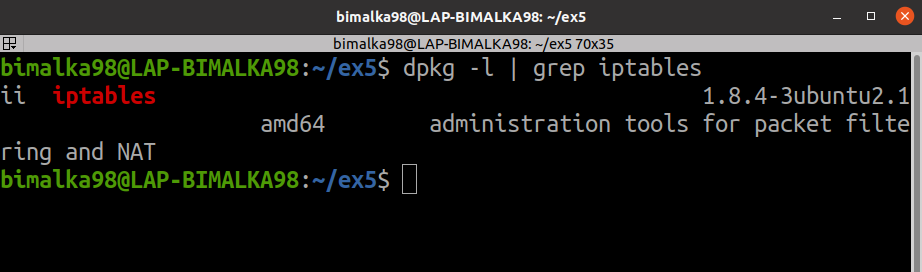
\includegraphics[width=0.65\columnwidth]{images/part1/2.png}
				\caption{Checking whether {\tt iptables} is installed on the system}
			\end{figure}
		\end{answer}
		
		\item Check all available iptables rules in your system using the command \texttt{/sbin/iptables -n -L }.
		
		\begin{answer}
			\begin{figure}[H]
				\centering
				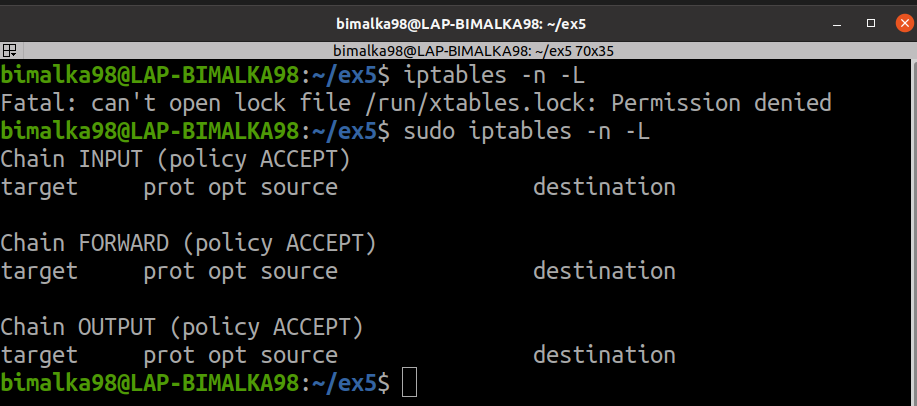
\includegraphics[width=0.65\columnwidth]{images/part1/3.png}
				\caption{Checking all available {\tt iptables} rules}
			\end{figure}
		\end{answer}
		
		\item Save all available iptables rules to a file named \textbf{iptablesRule.v4} using \texttt{iptables-save} command.
		
		\begin{answer}
			\begin{figure}[H]
				\centering
				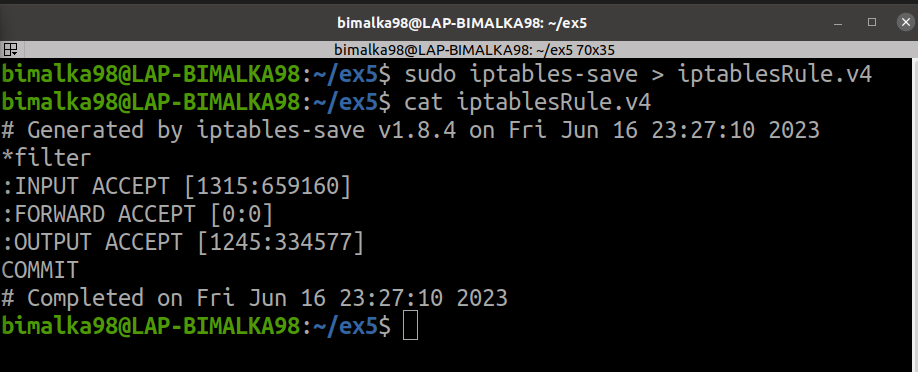
\includegraphics[width=0.65\columnwidth]{images/part1/4.png}
				\caption{Saving all available {\tt iptables} rules}
			\end{figure}
		\end{answer}
		
		\item Flush all the iptables rules that exist in your system and set a default policy to drop packets.
		\begin{answer}
			\begin{figure}[H]
				\centering
				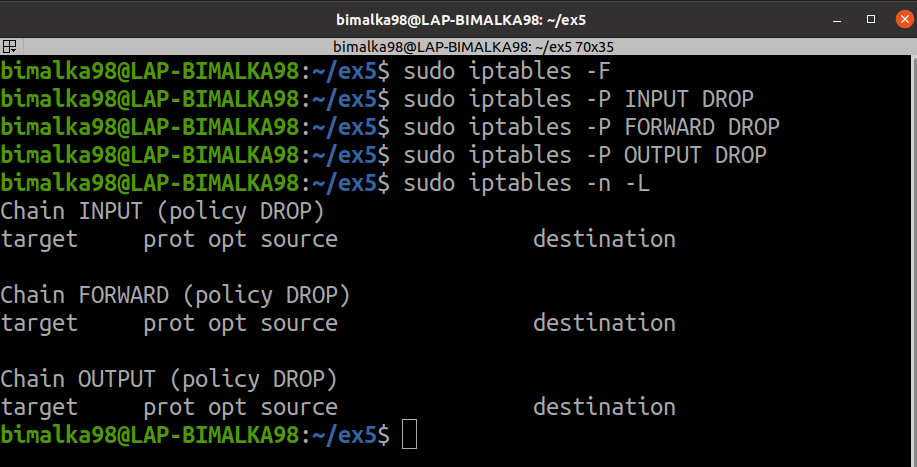
\includegraphics[width=0.65\columnwidth]{images/part1/5.png}
				\caption{Flushing all the rules and setting a default policy to drop packets}
			\end{figure}
		\end{answer}
		
		\item Set iptables rules to permit input and output DNS traffic in your system.
		
		\begin{answer}
			\begin{figure}[H]
				\centering
				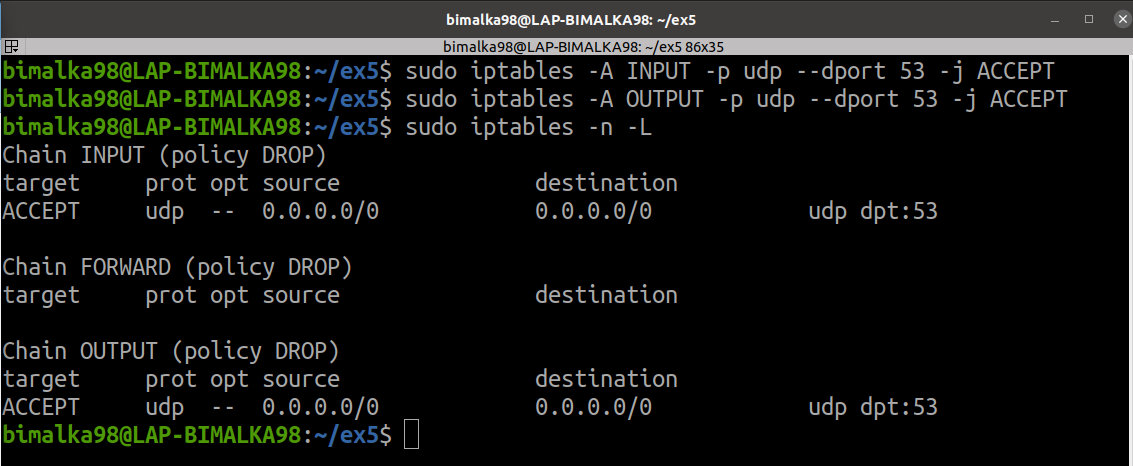
\includegraphics[width=0.65\columnwidth]{images/part1/6.png}
				\caption{Permitting input and output DNS traffic}
			\end{figure}
		\end{answer}
		
		\item Add iptables rules to accept local network incoming and outgoing traffic from the network 192.168.1.0/24. 
		\begin{answer}
			
			\begin{figure}[H]
				\centering
				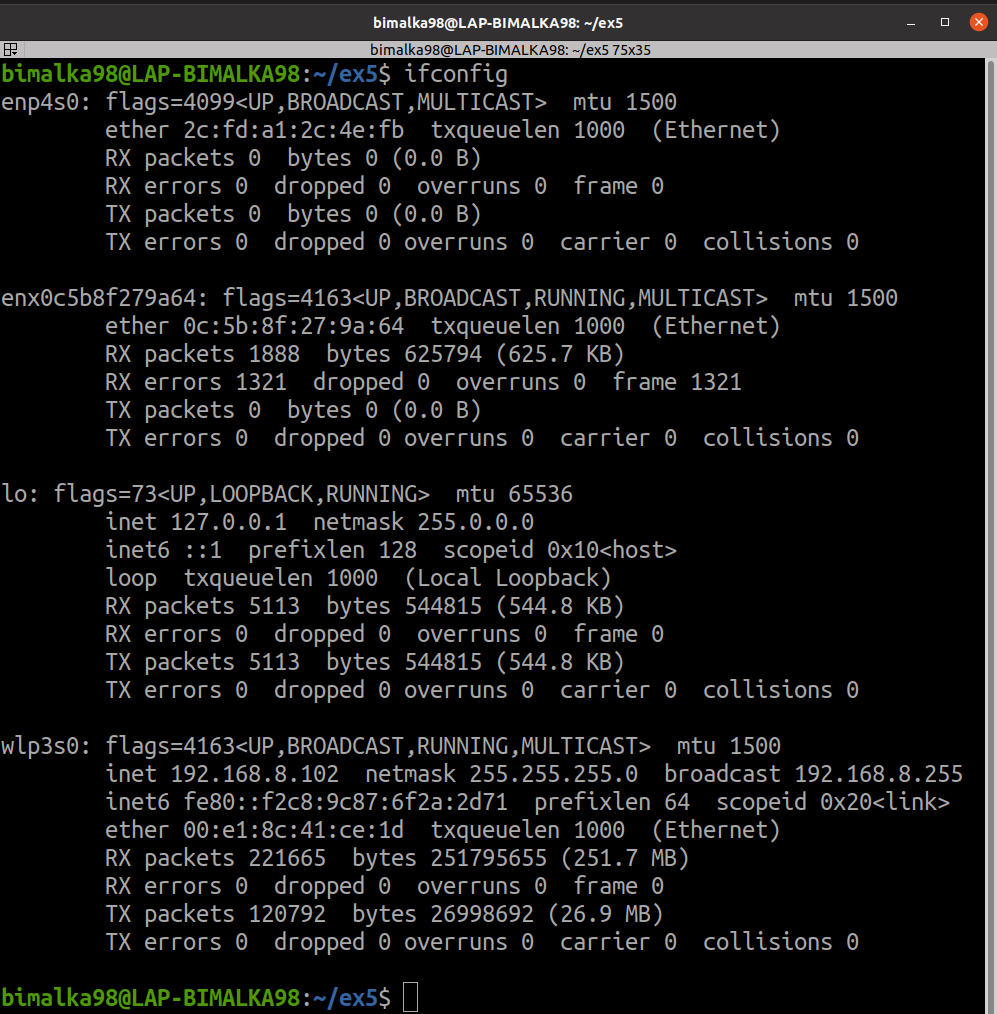
\includegraphics[width=0.65\columnwidth]{images/part1/ifconfig.png}
				\caption{Checking the CIDR of the current local network}
			\end{figure}
			
			\begin{figure}[H]
				\centering
				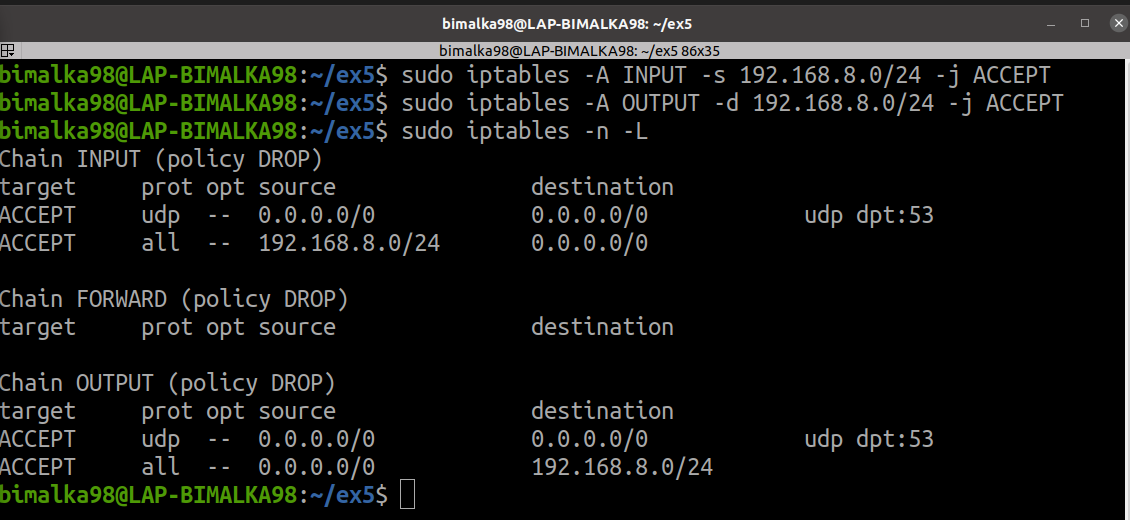
\includegraphics[width=0.65\columnwidth]{images/part1/7.png}
				\caption{Adding rules to accept local network incoming and outgoing traffic}
			\end{figure}
		\end{answer}
		\pagebreak
		\item Configure iptables rules to allow all HTTP traffic.
		\begin{answer}
			\begin{figure}[H]
				\centering
				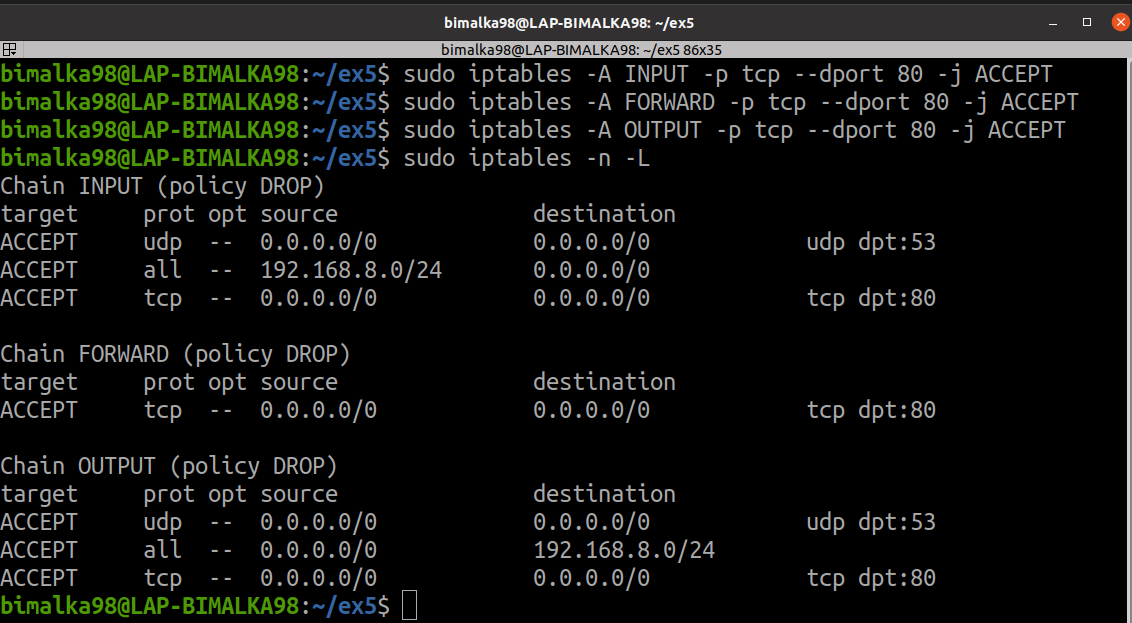
\includegraphics[width=0.65\columnwidth]{images/part1/8.png}
				\caption{Configuring rules to allow all HTTP traffic}
				\label{fig:8}
			\end{figure}
		\end{answer}
		
		\item View all iptables rules in your system and save them to a file \textbf{iptablesRuleNew.v4}. 
		\begin{answer}
			\begin{figure}[H]
				\centering
				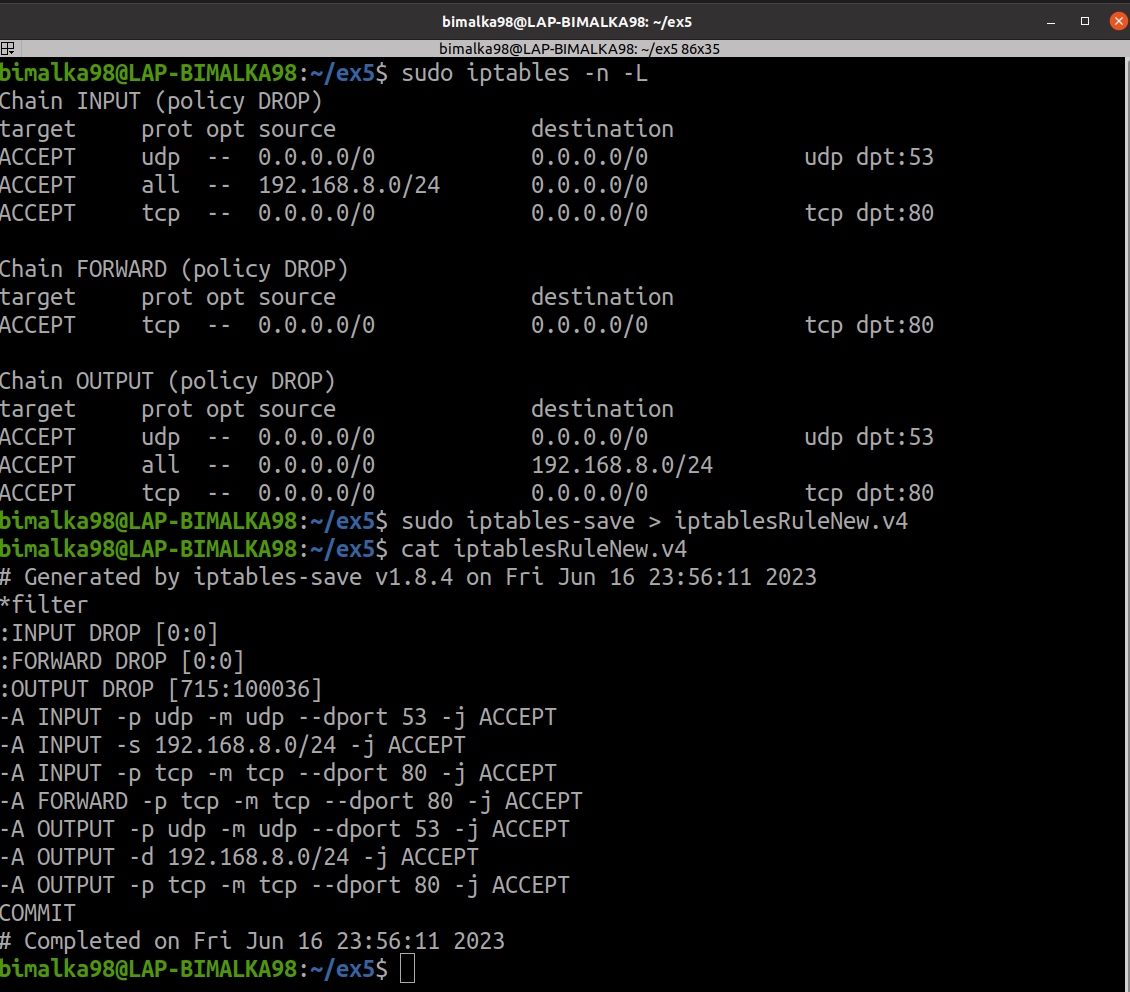
\includegraphics[width=0.65\columnwidth]{images/part1/9.png}
				\caption{Viewing all rules and saving them to a file}
			\end{figure}
		\end{answer}
		\pagebreak
		\item Create a file called \textbf{iptablesCommands.sh} and put all commands you ran from steps 4, 5 and 6 in the file. After creating the file, flush your iptables commands again and run \textbf{iptablesCommands.sh} file. View the iptables rules now and compare with the previous result.
		
		\begin{answer}
			\begin{figure}[H]
				\centering
				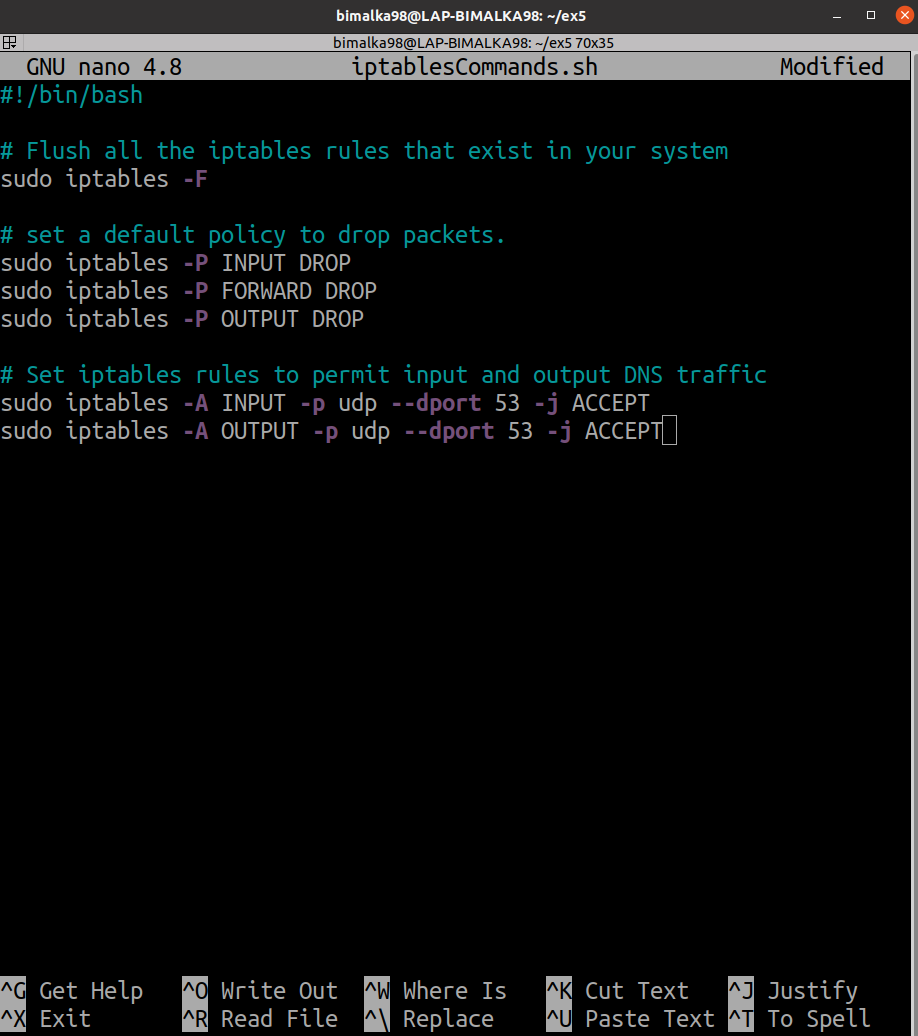
\includegraphics[width=0.65\columnwidth]{images/part1/10_1.png}
				\caption{Creating the shell script}
			\end{figure}
			
			\begin{figure}[H]
				\centering
				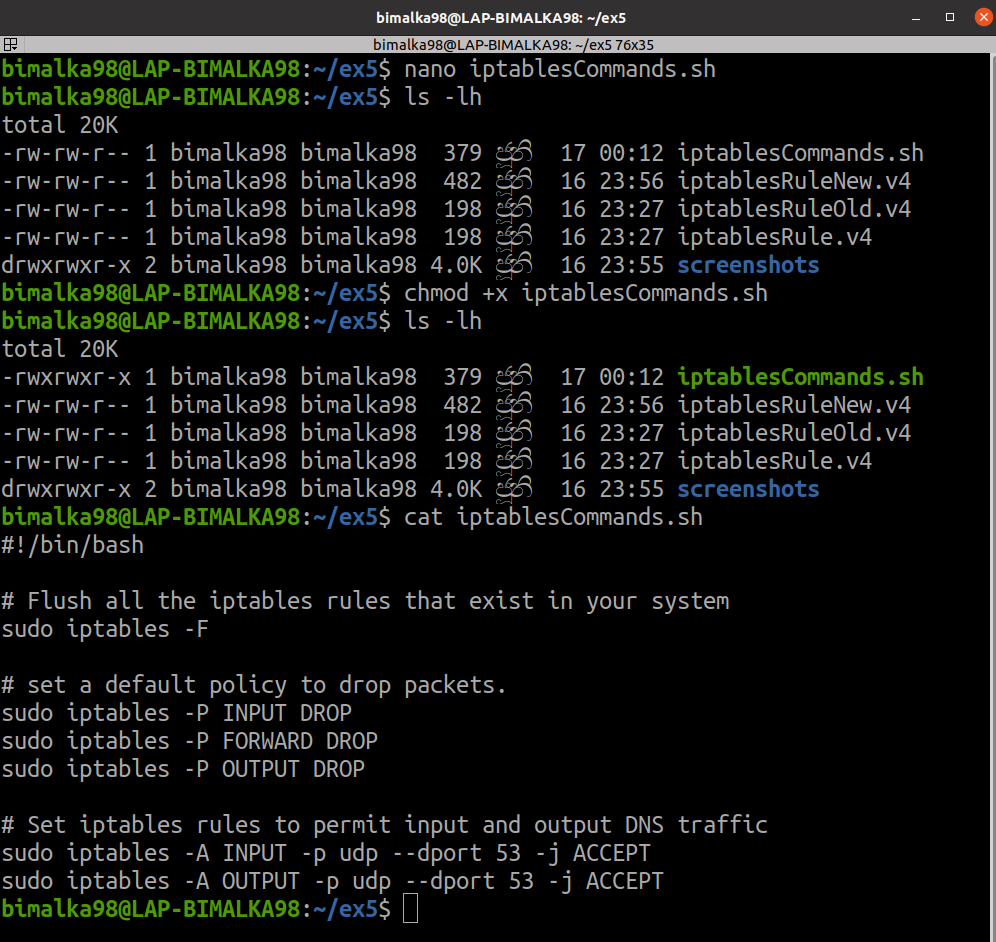
\includegraphics[width=0.65\columnwidth]{images/part1/10_2.png}
				\caption{Making the script executable}
			\end{figure}
		
			\begin{figure}[H]
				\centering
				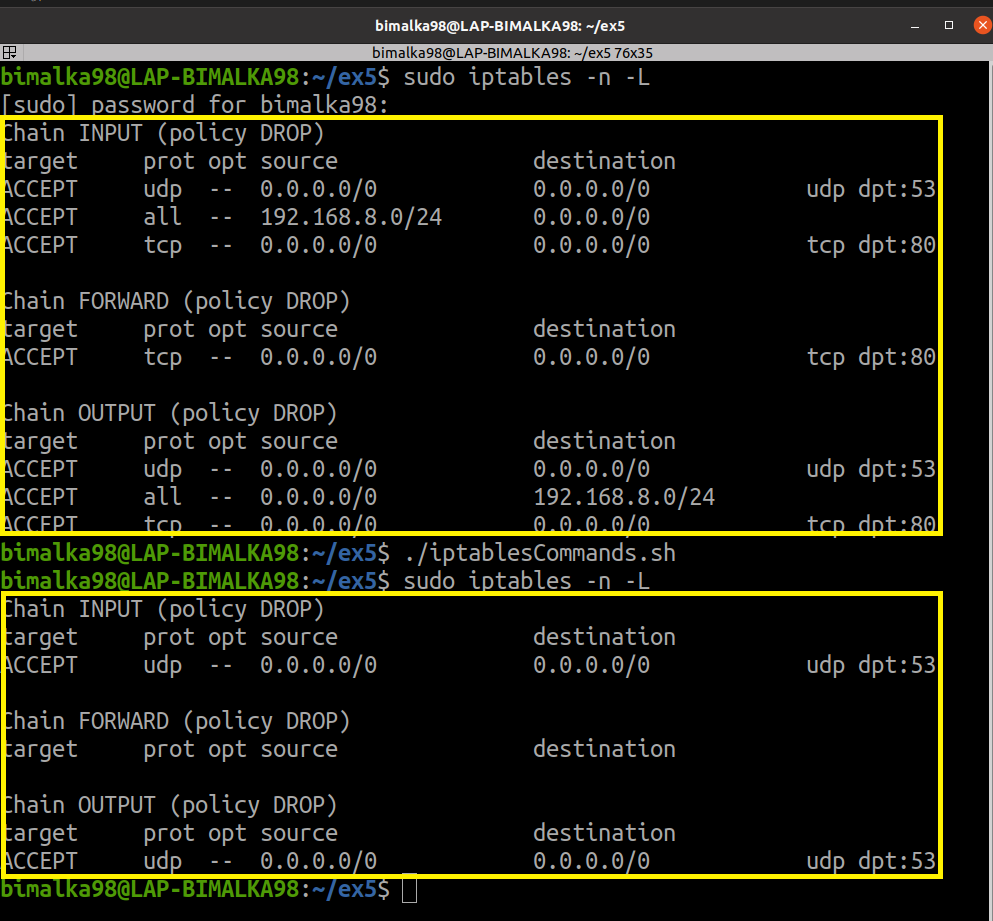
\includegraphics[width=0.65\columnwidth]{images/part1/10_3.png}
				\caption{Executing the shell script}
				\label{scripting}
			\end{figure}
		
		As it can be observed in the Figure \ref{scripting}, it is possible to set {\tt iptables} rules through shell scripts, which is an efficient way when it comes to setting rules in multiple host devices. In terms of the differences there is no difference between setting the rules manually and setting the rules through the script. The reason for the change in the number of rules is just because some rules were not included in the script (only the rules from item 4, 5 and 6 are there).
		\end{answer}
				
		\pagebreak
		\item Finally, flush your iptables rules again. But this time, load the saved iptables rules from the file \textbf{iptablesRuleNew.v4} using \texttt{iptables-restore} command. View the iptables rules and compare them with the ones you have in step 8.
		\begin{answer}
			\begin{figure}[H]
				\centering
				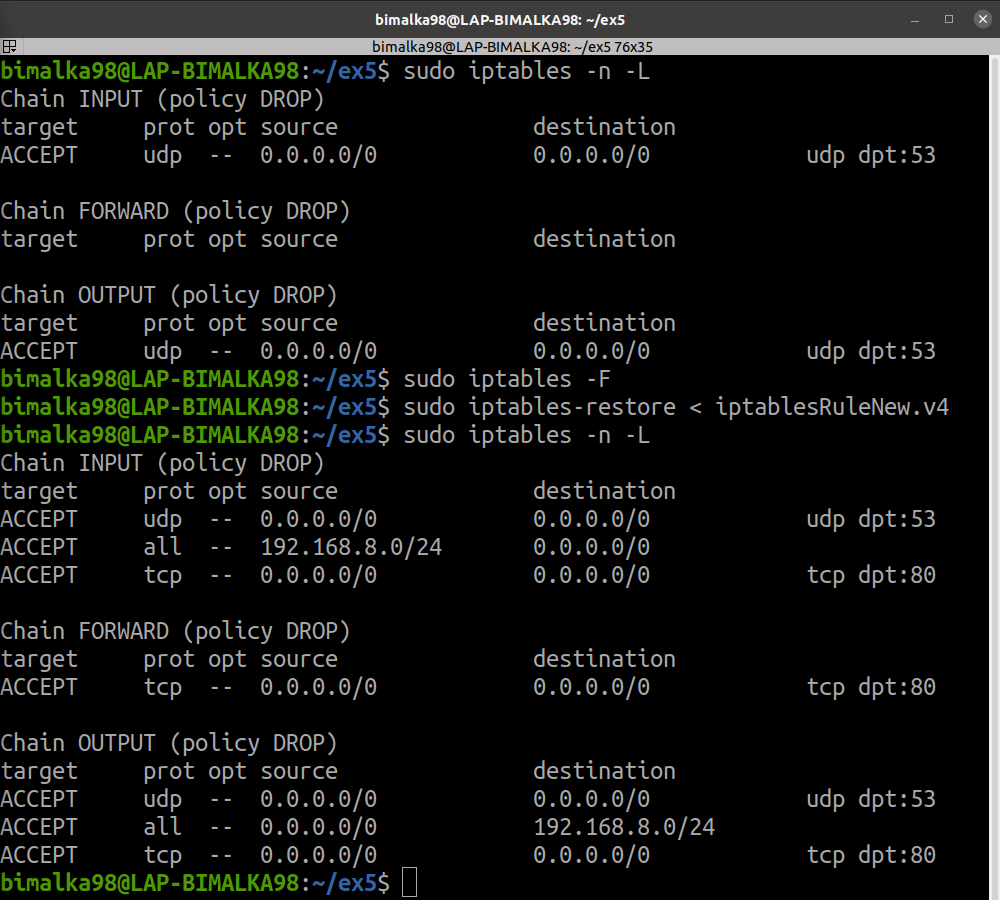
\includegraphics[width=0.65\columnwidth]{images/part1/11.png}
				\caption{Flushing current rules and restoring saved rules}
				\label{fig:11}
			\end{figure}
		
		When comparing the output shown in the Figure \ref{fig:11} and the Figure \ref{fig:8}, it can be observed that there is no difference. This means it is possible to save {\tt iptables} of a host at a given moment and restore them at another moment as required. This can be a useful tool when it comes to backing up rules before any significant change to the rules, because if anything goes wrong we have a fallback position.
		\end{answer}
		\pagebreak
		\subsubsection*{Creating Firewall Rules with UFW}
		
		The scenario comprises of two virtual machines (VM1 IP - 192.168.46.140 and VM2 IP - 192.168.46.141) running on a host (HOST IP - 192.168.46.1) machine. VM1 is an Ubuntu virtual machine that has a firewall implemented/configured. 
		
		The current firewall ruleset is as below.
		\begin{figure}[H]
			\centering
			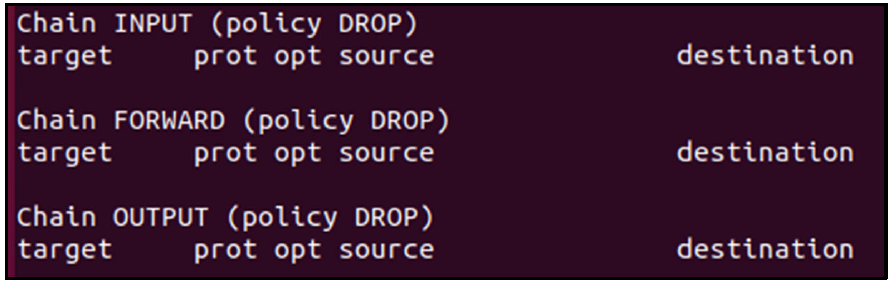
\includegraphics[width=0.5\columnwidth]{images/ex5-firewall-rules.png}
		\end{figure}
		
		All chain policies are set to drop traffic. To implement base rules, you can use the following commands:
		
		\begin{itemize}
			\item Delete any current rules associated with UFW using \texttt{sudo ufw reset}
			\item Disable UFW using \texttt{sudo ufw disable}
			\item Flush all iptables rules using \texttt{sudo iptables -F}
			\item Enable UFW using \texttt{sudo ufw enable}
			\item Deny outgoing traffic using \texttt{sudo ufw default deny outgoing}
		\end{itemize}
	
		\begin{figure}[H]
			\centering
			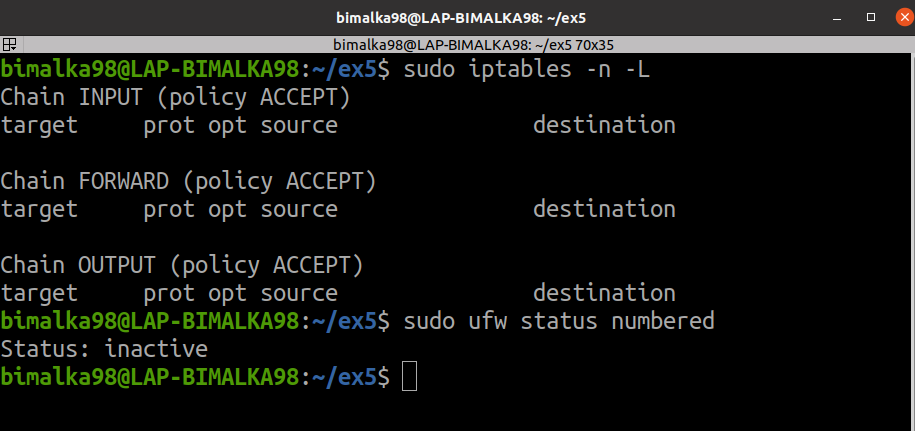
\includegraphics[width=0.75\columnwidth]{images/part2/1.png}
			\caption{Current firewall rules}
		\end{figure}
		
		\begin{figure}[H]
			\centering
			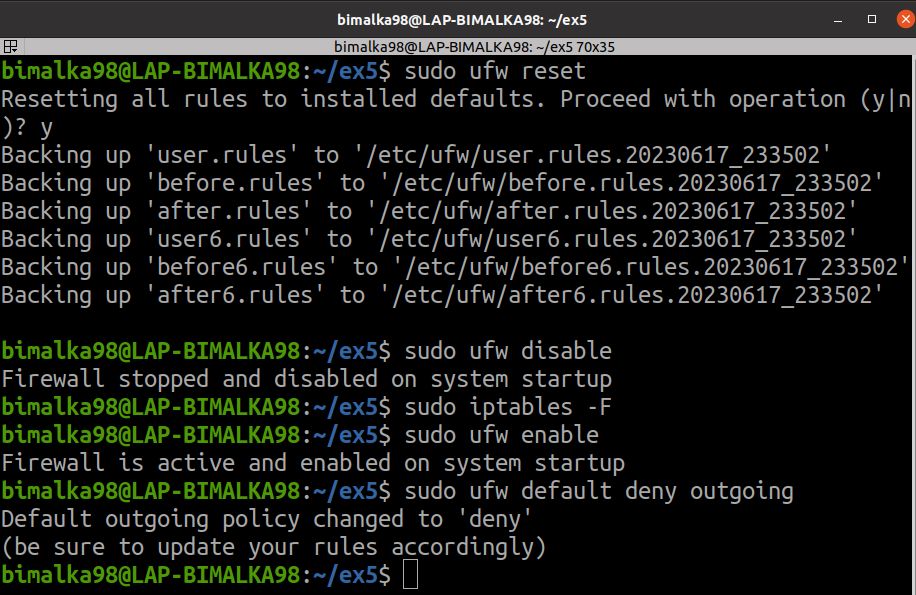
\includegraphics[width=0.75\columnwidth]{images/part2/2.png}
			\caption{Implementing the base rules}
		\end{figure}
		
		\begin{figure}[H]
			\centering
			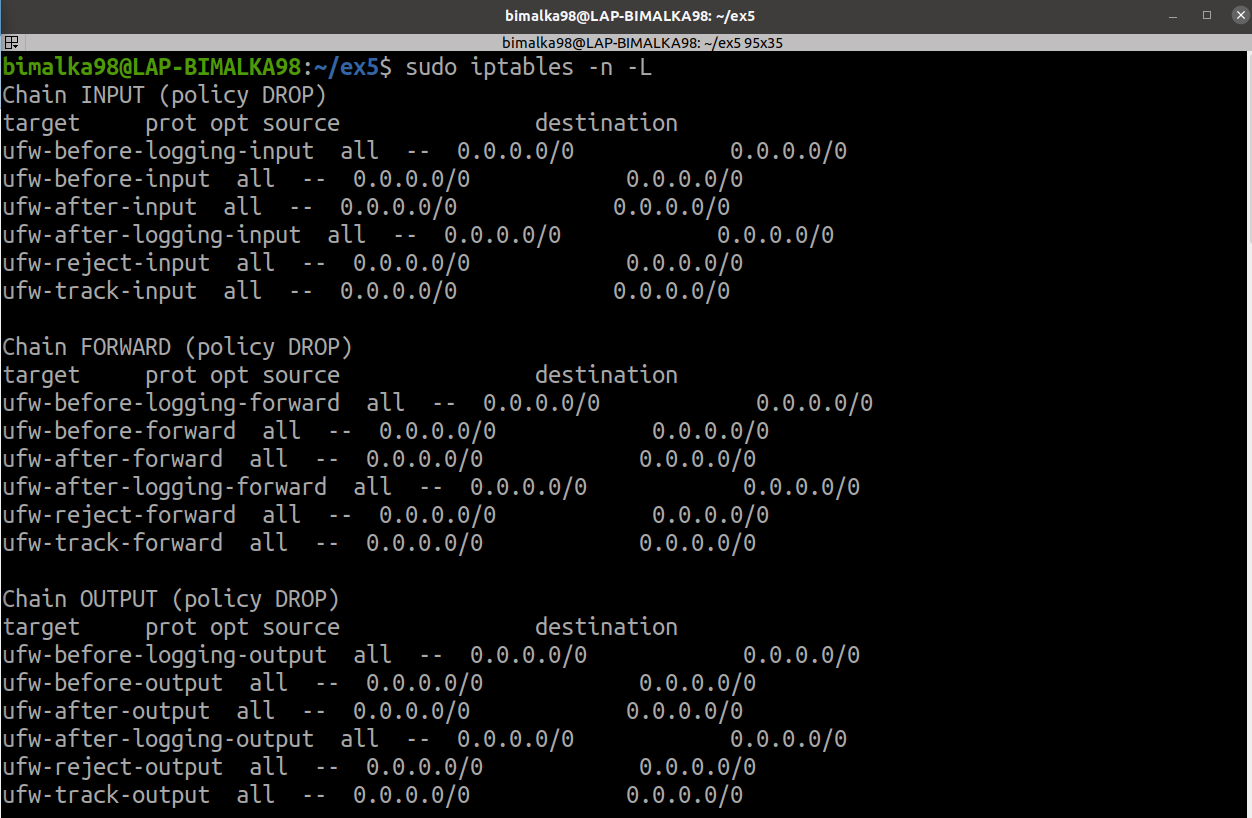
\includegraphics[width=0.75\columnwidth]{images/part2/3.png}
			\caption{{\tt iptables} after setting up the base rules}
		\end{figure}
		\pagebreak
		\item Implement the following network administration in VM1:
		\begin{itemize}
			\item Access to VM1 from VM2 must only be allowed over FTP and Telnet.
			\item Access to VM1 from HOST must only be allowed over SSH
			\item Allow all outgoing traffic from VM1 with the exception of access to HTTP websites
		\end{itemize}
		
		In this task, you are asked to implement UFW rules on the ubuntu machine. You can pretend that VM2 and HOST exist in your network. List the commands you used to achieve the above. Add a screenshot of the terminal output after running the command \texttt{sudo ufw status numbered}.
		
		If the firewall is physically implemented, you could have tested the connections using PuTTY or the command line.
		
		\begin{answer}			

			Following network administration in VM1 is configured using the associated commands given below.
			\begin{itemize}
				\item Access to VM1 from VM2 must only be allowed over FTP and Telnet
				\begin{verbatim}
					sudo ufw allow in from 192.168.46.141 to any port 21 proto tcp
					sudo ufw allow in from 192.168.46.141 to any port 23 proto tcp
				\end{verbatim}
			
				\item Access to VM1 from HOST must only be allowed over SSH
				
				\begin{verbatim}
					sudo ufw allow in from 192.168.46.1 to any port 22 proto tcp
				\end{verbatim}
				
				\item Allow all outgoing traffic from VM1 with the exception of access to HTTP websites
				
				\begin{verbatim}
					sudo ufw default allow outgoing					
					sudo ufw deny out to any port 80 proto tcp
				\end{verbatim}
			\end{itemize}
		
		
			\begin{figure}[H]
				\centering
				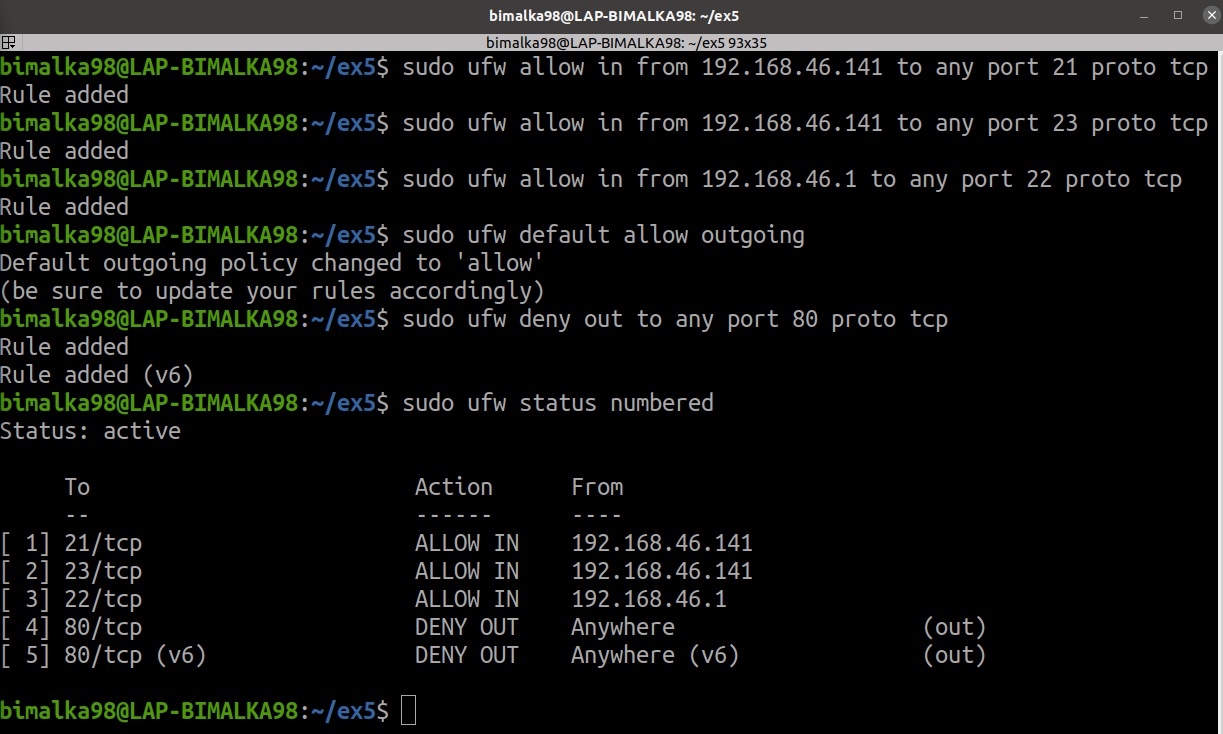
\includegraphics[width=0.75\columnwidth]{images/part2/4.png}
				\caption{Output after running the command \texttt{sudo ufw status numbered}}
			\end{figure}
		
			\begin{figure}[H]
				\centering
				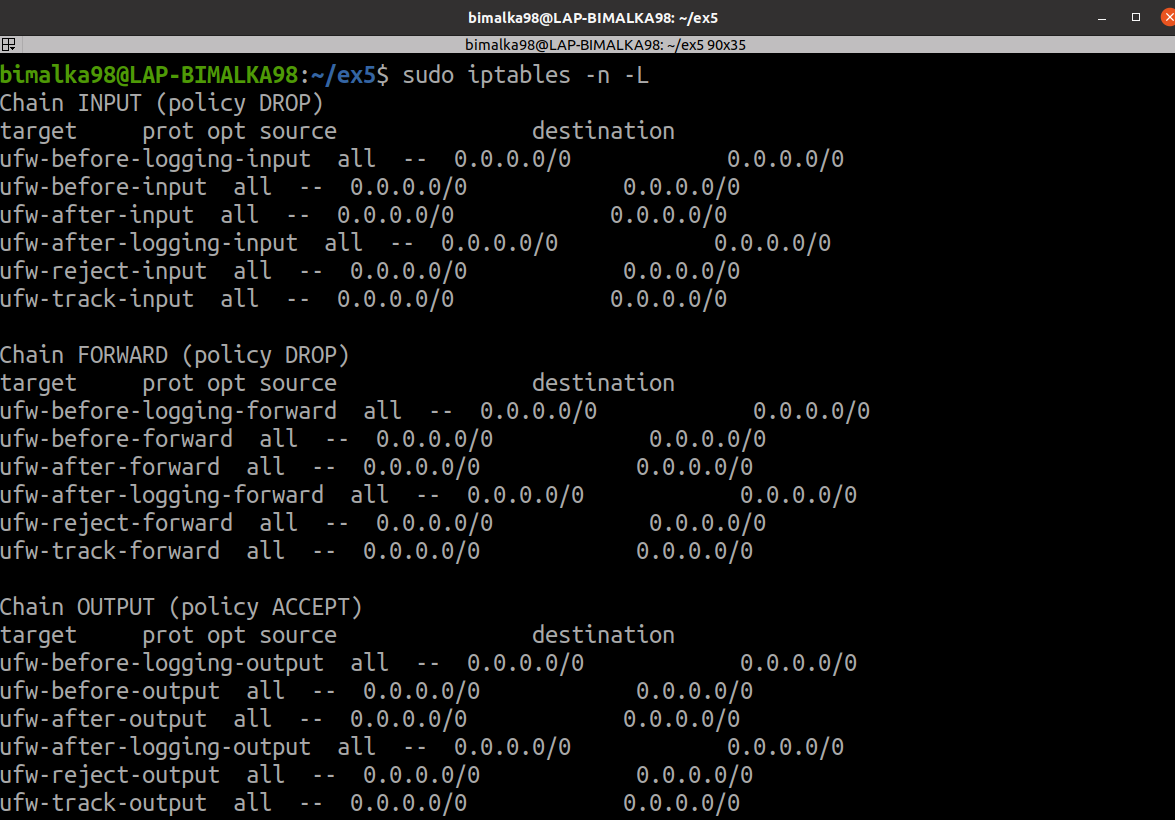
\includegraphics[width=0.75\columnwidth]{images/part2/5.png}
				\caption{{\tt iptables} ruleset after mentioned configurations}
			\end{figure}
		
			\begin{figure}[H]
				\centering
				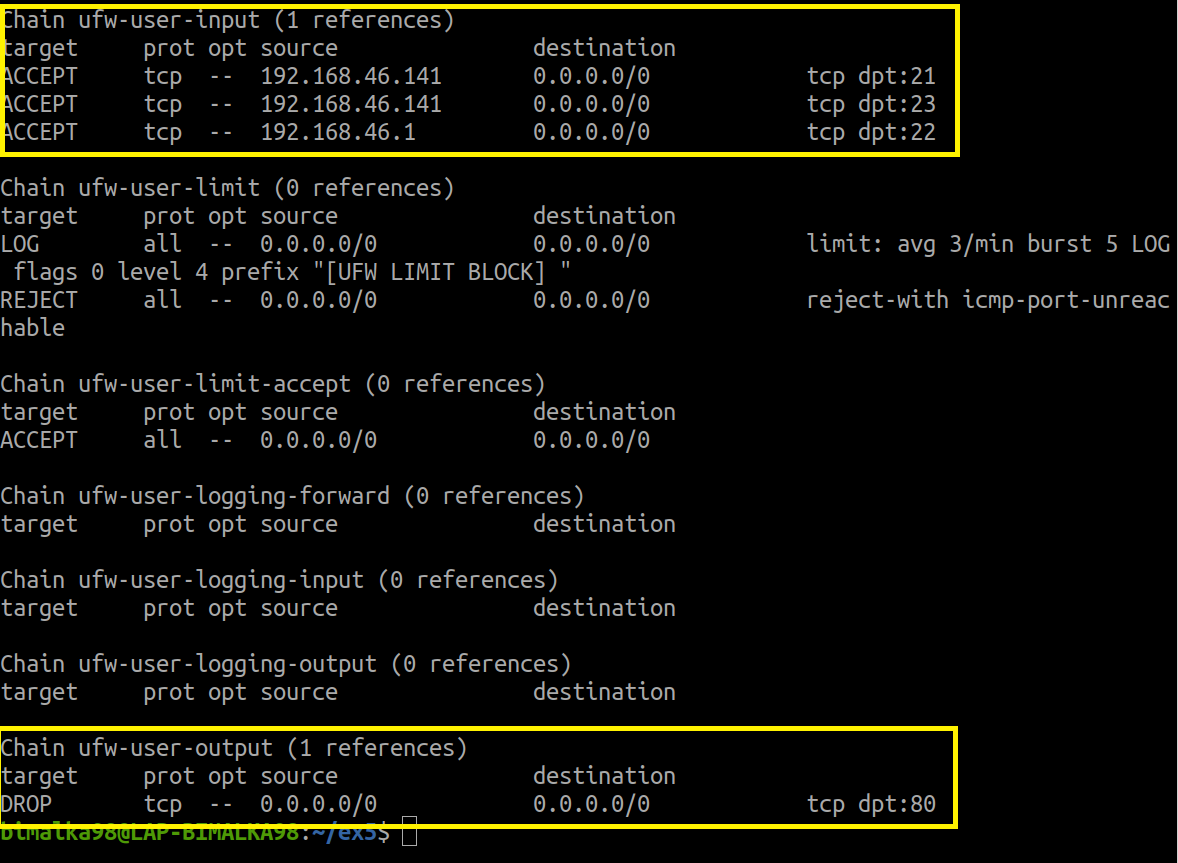
\includegraphics[width=0.75\columnwidth]{images/part2/6.png}
				\caption{Mentioned configurations in the {\tt iptables}}
			\end{figure}
		\end{answer}
		\pagebreak
		\subsubsection*{Scan systems with NMAP}
		In this section, you will scan for the Ports of a remote host. You will need to have two devices connected to the same local network to perform this task. 
		
		\item View ip addresses of both devices using \texttt{hostname -I} command.
		\begin{answer}
			\begin{figure}[H]
				\centering
				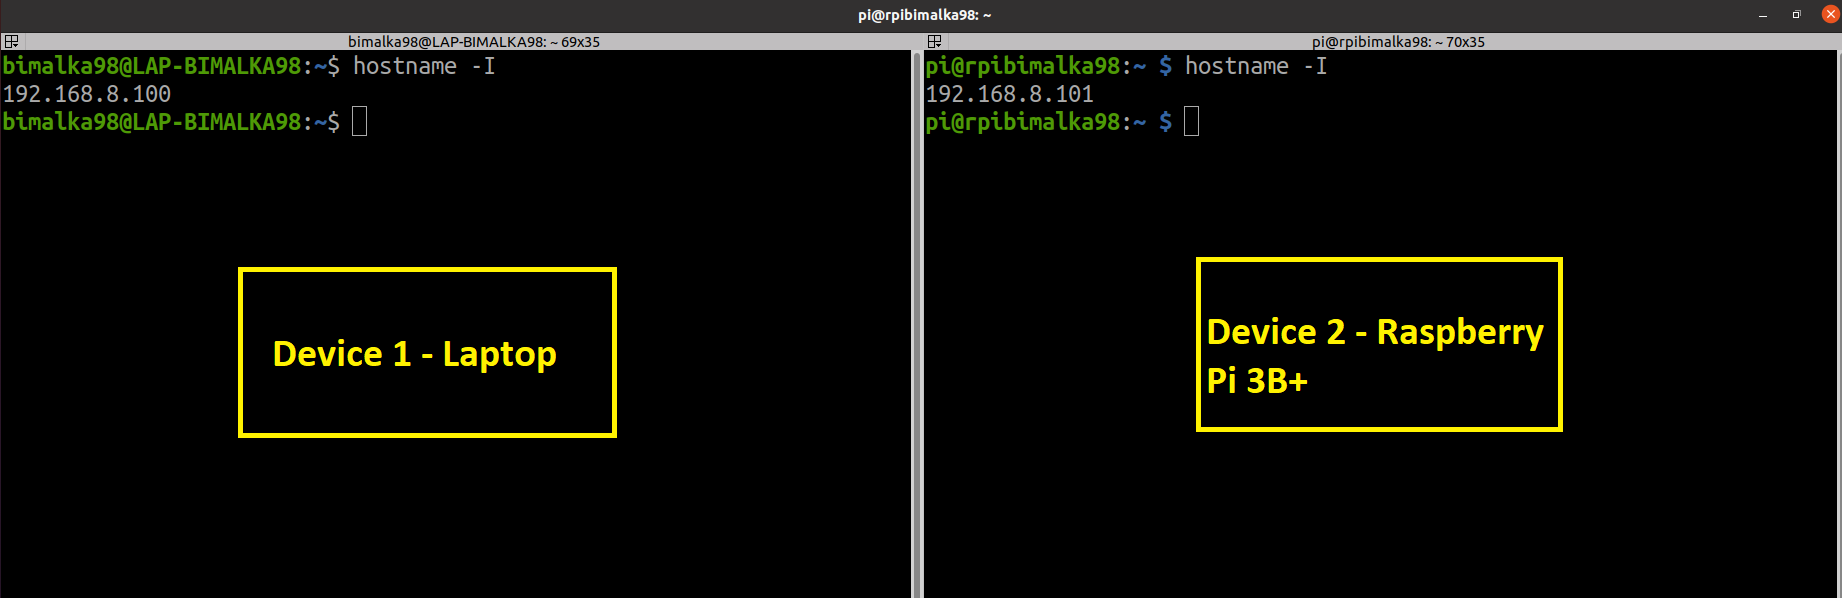
\includegraphics[width=0.9\columnwidth]{images/part3/2.png}
				\caption{IP addresses of the two devices (Laptop \& a Raspberry Pi)}
			\end{figure}
		\end{answer}
		\item Scan one host from the other host for TCP and UDP ports using \texttt{nmap} command.
		\begin{answer}
			\begin{figure}[H]
				\centering
				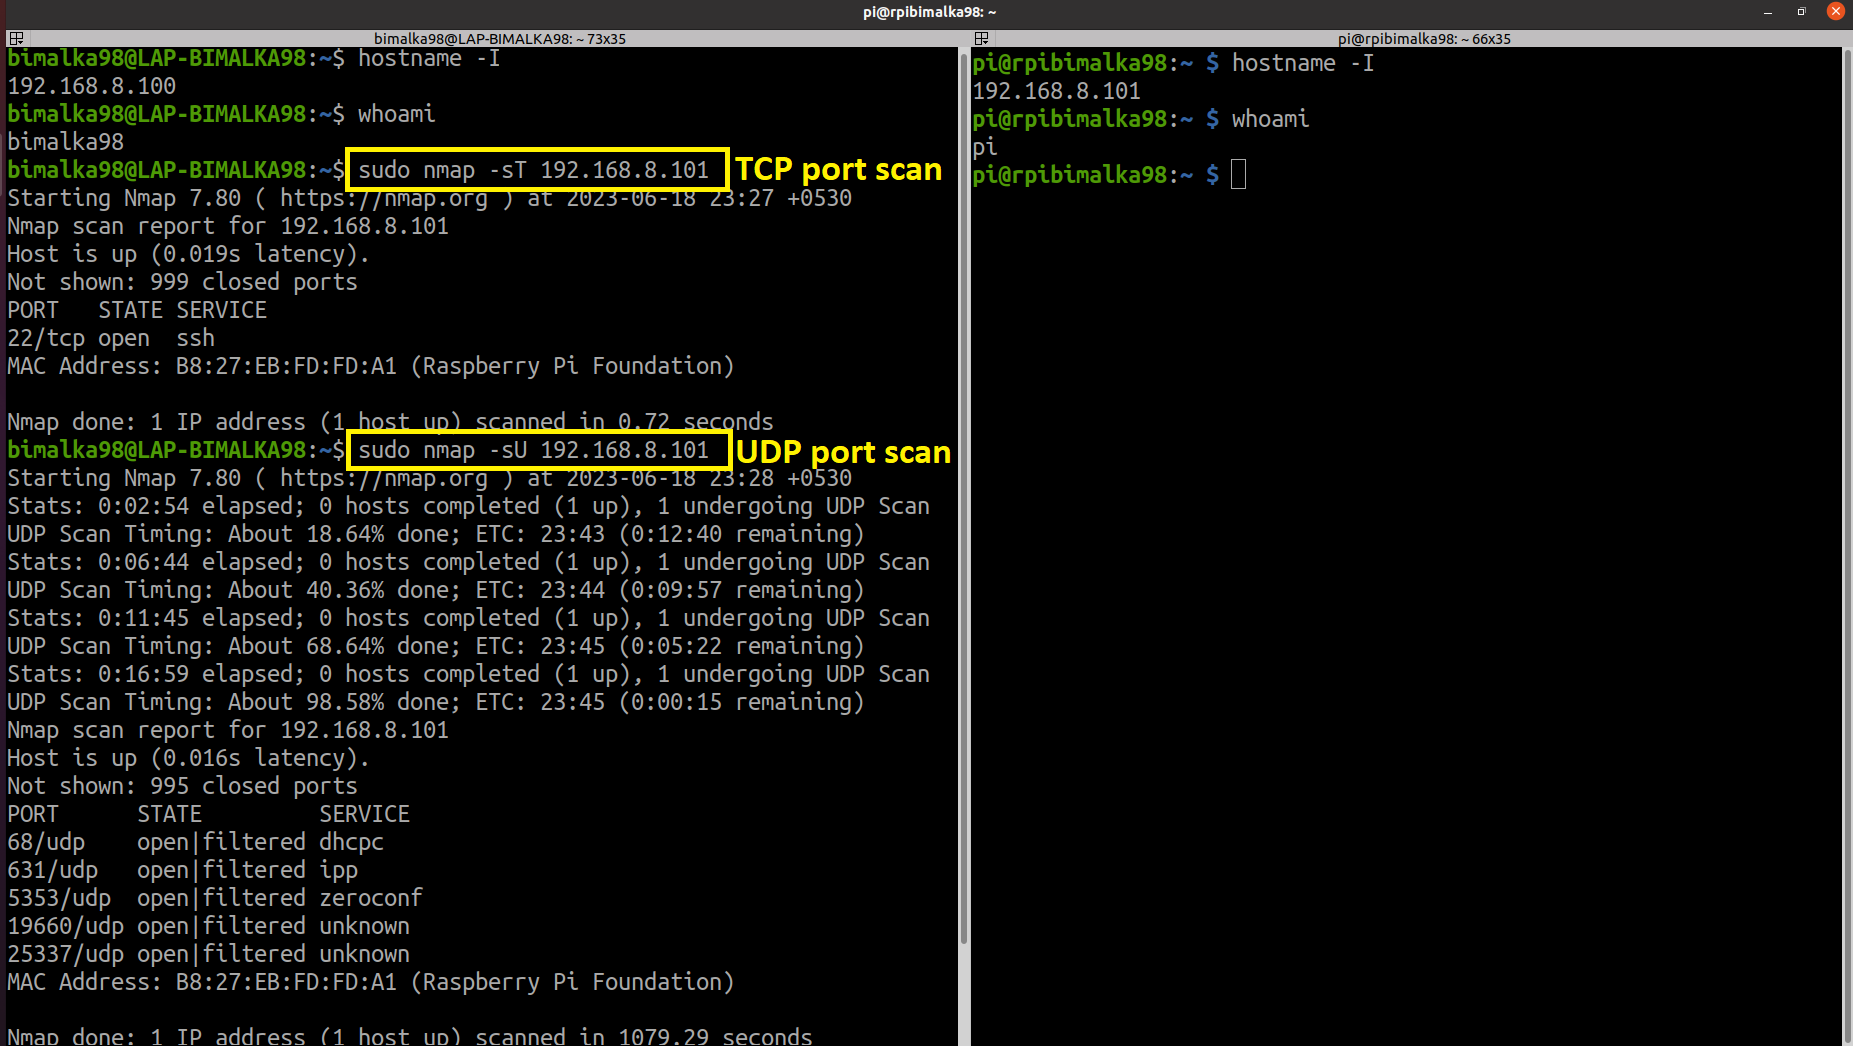
\includegraphics[width=0.9\columnwidth]{images/part3/4.png}
				\caption{Scan Raspberry Pi device from the Laptop for TCP and UDP ports}
			\end{figure}
		\end{answer}
		
		\section*{Section 2}
		
		
		\item Briefly explain VLANs, VPNs, DMZs and Network Segmentation concepts outlining their similarities and differences.
		
		\begin{answer}
			\textbf{VLAN (a virtual local area network} allows multiple logical networks to exist on the same physical network. This improves the security and the performance of a given network by limiting the access to the resources within the given VLAN and isolating the traffic of a given VLAN from other VLANs respectively. VLANs assigned for each department of an organization is an example for this.\\
			
			\textbf{VPN (a virtual private network)} allows an encrypted tunnel to be created between two end points in an unsecured network (eg: internet) for secure communication. This minimize the possibility of being tracked by a malicious third party. VPNs are used to connect remote employees or branches of an organization, to its corporate network for secure communication.\\
			
			\textbf{DMZ (a demilitarized zone)} or otherwise known as a perimeter network/ screened subnet is a physical or logical network segment (a buffer) that separates an organization's internal LAN from the other unsecured networks (eg: internet). This allows an additional layer of security to be maintained, as it restrict the direct access from the internet to the LAN. The services/ servers provided to public are placed in the DMZ, while organization's private resources are kept in the internal network.\\
			
			\textbf{Network Segmentation} is a method to isolate/ control the traffic of a given network. As in the VLANs, improved performance due to reduced traffic congestion and improved security due to virtual isolation of networks are the benefits.\\		
		\end{answer}
		
		\item Perform a comparison between IPsec and SSL.
		
		Answer was adapted from:\\ \url{https://www.geeksforgeeks.org/difference-between-ipsec-and-ssl/}
		
		\begin{table}[htbp]
			\centering
			\caption{Comparison of IPsec and SSL}
			\begin{tabularx}{0.9\columnwidth}{|X|X|}
				\hline
				\textbf{IPsec} & \textbf{SSL}\\
				\hline
				\textcolor{blue}{A set of protocols that provide security for IP (Internet Protocol) protocol} & 
				\textcolor{blue}{A protocol developed for secure communication} \\  
				\hline 
				\textcolor{blue}{Operates in the \textit{Internet/ Network} layer of the TCP/IP stack} & 
				\textcolor{blue}{Operates in between \textit{Transport} and \textit{Application} layers of the TCP/IP stack} \\ 
				\hline 
				\textcolor{blue}{Used in securing VPNs} & 
				\textcolor{blue}{Used in securing web transactions} \\ 
				\hline
				\textcolor{blue}{Involves a complex configurations } & 
				\textcolor{blue}{Comparatively less complex to set up } \\ 
				\hline
				\textcolor{blue}{Installation is not specific to the vendor} & 
				\textcolor{blue}{Installation is specific to the vendor} \\ 
				\hline
				
			\end{tabularx}
		\end{table}
		\pagebreak
		\item Explain the differences between an IDS, an IPS, and a firewall?
		
		\begin{answer}
			 An IDS (Intrusion Detection System)  is a passive network monitoring system, which is only capable of detecting threats and alerting the network administrator or the SOC (the security operations center).\\
			 
			 Whereas IPS (Intrusion Prevention System) is an active network monitoring system which not only detect the threats, but also take actions to prevent or block them in real time. This is done through analyzing the traffic and checking them against known attack patterns or policies of the network.\\
			 
			 In contrast to the above a firewall provides a general protection by simply controlling the access to a given network, based on predefined set of rules. This can include the rules to allow or block traffics from a given subnet, allow or block traffics through a specific port and etc.
		\end{answer}
		
		\item What is the difference between anomaly detection and signature or heuristic-based intrusion detection?
		
		\begin{answer}
			%% TODO: Add answer here
			Your answer here
		\end{answer}
		
	\end{enumerate}
	
\end{document}